
\documentclass[12pt,hyperref={CJKbookmarks=true}]{beamer} %14pt为字体尺寸,默认值11pt.有8-12;14;17;20;bigger;smaller
%%%%%%%%%%%%%%%%%%%%%%%%%%%%%%%%%%%%%%%%%
% 模板資訊:
% 模板名稱:Beamer
% 版本:1.0 (2023.07.09)
% 修改者:Ernie
% 編譯器:XeLaTeX
%
% 原始模板的資訊:
% 模板名稱:Beamer Presentation
% 作者:Vel (vel@latextemplates.com)
% 編譯器:XeLaTeX
% 授權:CC BY-NC-SA 4.0 (https://creativecommons.org/licenses/by-nc-sa/4.0/)
% 下載連結:https://www.LaTeXTemplates.com
%
% 製作本模板之目的:
% 為了讓 LaTeX 初學者能夠輕鬆地完成專業的學術簡報,因此我針對 Vel 製作的模板做了大幅度的修改及附上清楚明瞭的註解。
%
% 如果您有任何問題,可以透過 Email 聯繫我們:stateconlab@gmail.com
% 
% p.s. 也別忘了關注我們的 YouTube、IG 和 Medium 喔!
% 1. YouTube:https://www.youtube.com/@StatEconLab
% 2. IG:https://www.instagram.com/stateconlab
% 3. Mediun:https://medium.com/@stateconlab
%%%%%%%%%%%%%%%%%%%%%%%%%%%%%%%%%%%%%%%%%

%----------------------------------------------------------------------------------------
%	封包與文檔配置
%----------------------------------------------------------------------------------------

\usepackage[space,noindent]{ctex}

% 自訂字體顏色的封包
\usepackage{xcolor} 

%% 自訂顏色

\definecolor{pbblue}{HTML}{0A75A8}% color for the progress bar and the circle
% 數學工具及符號
%\usepackage{mathtools, amsmath, amsfonts, amsthm, latexsym} 

% 分別將數學符號間的間隔加大及加粗
%\usepackage{newtxtext,newtxmath}

% 圖表自動編號的封包
%\usepackage{caption} 

%% 設定自動編號
%\setbeamertemplate{caption}[numbered]

%% 設定圖表編號及標籤的字體大小及字形
%\captionsetup[figure]{font=small, labelfont=md}
%\captionsetup[table]{font=small, labelfont=md}

% 導入圖形與表格的封包
%\usepackage{graphicx}  % \scalebox{} 可用於將過大的表格縮小
%\usepackage{booktabs}

% 排列多個子圖形的封包
%\usepackage{subfigure} 

% 允許表格的一格能多列呈現的封包
%\usepackage{multirow} 

% 可指定表格排版的封包
%\usepackage{array}

% 翻轉表格的封包
%\usepackage{lscape} 

% 序列標號
%\usepackage{enumerate} 

% 繪圖封包 (用於添加浮水印)
\usepackage{tikz}

% 引注參考資料
%\usepackage{natbib}

% 註釋掉大部分的封包
%\usepackage{comment}

\usetikzlibrary{shapes,fit,calc,positioning}

% 設定中文的標籤
%\renewcommand{\figurename}{圖} 
\renewcommand{\tablename}{表} 

%----------------------------------------------------------------------------------------
%	排版形式 (擇一,不選等同選擇默認的排版形式)
%----------------------------------------------------------------------------------------

%\mode<presentation>{
%\usetheme{default}
%\usetheme{AnnArbor}
%\usetheme{Antibes}
%\usetheme{Bergen}
%\usetheme{Berkeley}%演示主题为侧边导航条
%\usetheme{Berlin}
\usetheme{Boadilla}%蓝色主题
%\usetheme{CambridgeUS}
%\usetheme{Copenhagen}
%\usetheme{Darmstadt}
%\usetheme{Dresden}
%\usetheme{Frankfurt}
%\usetheme{Goettingen}
%\usetheme{Hannover}
%\usetheme{Ilmenau}
%\usetheme{JuanLesPins}
%\usetheme{Luebeck}
%\usetheme{Madrid}
%\usetheme{Malmoe}
%\usetheme{Marburg}
%\usetheme{Montpellier}
%\usetheme{PaloAlto}
%\usetheme{Pittsburgh}
%\usetheme{Rochester}
%\usetheme{Singapore}
%\usetheme{Szeged}
%\usetheme{Warsaw}

%----------------------------------------------------------------------------------------
%	外框形式 (擇一,不選等同選擇默認的外框形式)
%----------------------------------------------------------------------------------------

%\useoutertheme{default}
%\useoutertheme{infolines}
%\useoutertheme{miniframes}
%\useoutertheme{smoothbars}
%\useoutertheme{sidebar}
%\useoutertheme{split}
%\useoutertheme{shadow}
%\useoutertheme{tree}
%\useoutertheme{smoothtree}

%----------------------------------------------------------------------------------------
%	外框的自訂義調整 
%----------------------------------------------------------------------------------------

% 外框上緣的字 (fg) 為黑色,背景 (bg) 為白色。
%\setbeamercolor{section in head/foot}{fg=white, bg=black} 

% 外框上緣顯示的章節(section)頁數標籤是否關閉
%\setbeamertemplate{mini frames}{}   

% 調整外框形式的字體大小
%\setbeamerfont{headline}{size=\scriptsize}
%\setbeamerfont{footline}{size=\scriptsize}

% 取消右下方的跳轉工具列
\setbeamertemplate{navigation symbols}{} 

%% 自定義1:外框下緣僅出現名字及頁碼
%\setbeamertemplate{footline}
%{\leavevmode%
%\hbox{%
%\begin{beamercolorbox}[wd=0.5\paperwidth,ht=3ex,dp=1ex,leftskip=2ex]%
%{author in head/foot}%
%{\footnotesize\textbf{\insertshortauthor}}%
%\end{beamercolorbox}%
%\begin{beamercolorbox}[wd=0.5\paperwidth,ht=3ex,dp=1ex,right]%
%{author in head/foot}%
%\footnotesize \textbf{{\insertframenumber{} / \inserttotalframenumber\hspace*{2ex}}} %頁碼控制選項
%\end{beamercolorbox}%
%}}

%% 自定義2:清除外框下緣但僅出頁碼
%\setbeamertemplate{footline}[page number] 

%% 自定義3:清除外框下緣
%\setbeamertemplate{footline}[] 

%----------------------------------------------------------------------------------------
%	顏色主題 (擇一,不選等同選擇默認的顏色主題)
%----------------------------------------------------------------------------------------

%\usecolortheme{default}
%\usecolortheme{albatross}
%\usecolortheme{beaver}
%\usecolortheme{beetle}
%\usecolortheme{crane}
%\usecolortheme{dolphin}
%\usecolortheme{dove}
%\usecolortheme{fly}
%\usecolortheme{lily}
%\usecolortheme{orchid}
%\usecolortheme{rose}
%\usecolortheme{seagull}
%\usecolortheme{seahorse}
\usecolortheme{whale}%颜色主题为
%\usecolortheme{wolverine}

%----------------------------------------------------------------------------------------
%	顏色主題的自訂義調整 
%----------------------------------------------------------------------------------------

% 全文的主題色 (可以特別針對報告對象或機構的代表色調整!)
%\setbeamercolor{structure}{fg=Myblue} 

% 封面頁中標題區塊的底色及字體顏色
%\setbeamercolor{title}{bg=green, fg=black} 

% 各頁標題區塊的底色及字體顏色
%\setbeamercolor{frametitle}{bg=white,fg=black} 

% 全文的內文顏色
%\setbeamercolor{normal text}{fg=orange}

% 數學區塊的標題顏色 
%\setbeamercolor{block title}{bg=blue,fg=yellow} 

% 數學區塊的內文顏色 
%\setbeamercolor{block body}{bg=green,fg=red} 

% 警示文字的顏色
%\setbeamercolor{alerted text}{fg=red} 

%----------------------------------------------------------------------------------------
%	enumerate 及 item 的形狀
%----------------------------------------------------------------------------------------

%\useinnertheme{rounded} % 圓球 (3D)
%\useinnertheme{circles} % 圓形 (2D)
%\useinnertheme{rectangles} % 方形
%\useinnertheme{triangle} % 三角形
%\useinnertheme{inmargin} % 插入邊沿
%\setbeamertemplate{itemize items}[triangle]

%----------------------------------------------------------------------------------------
%	自訂 item 的顏色
%----------------------------------------------------------------------------------------

%\setbeamercolor{item projected}{bg=red}

%----------------------------------------------------------------------------------------
%	個人化的設置及細節調整
%----------------------------------------------------------------------------------------

% 設定頁面邊界
%\setbeamersize{text margin left=0.6cm, text margin right=0.6cm}
%\special{papersize=\the\paperwidth,\the\paperheight}
%\providecommand{\tabularnewline}{\\}
%}

%----------------------------------------------------------------------------------------
%	個人化的背景調控
%----------------------------------------------------------------------------------------

% 背景照片設置
%\setbeamertemplate{background}{\includegraphics[height=\paperheight]{Fig/Background.png}}

% 浮水印設定
%\usebackgroundtemplate{%
%	\tikz[overlay, remember picture] % 讓 logo 能每頁都顯示
%	\node[opacity=0.3, below=-1.25cm, at=(current page.center)] % 調整透明度 (opacity) 及浮水印的位置
%	{\includegraphics[scale = 0.14]{Fig/nthulogo.png}}; % 載入 logo 及調整大小
%	}
 % 載入封包與文檔配置
% 参考文献样式
% 使用biblatex-gb7714-2015宏包提供的\footfullcite命令实现脚注引用。
\usepackage[backend=biber,autolang=hyphen,style=gb7714-2015,
gbtype=true,gbalign=gb7714-2015,
doi=false,url=false,isbn=false]{biblatex}
\tikzset{
dpu/.style={rectangle,rounded corners=2pt,
minimum width=35pt,minimum height=40pt,inner sep=5pt,
draw=black,fill=black!20,scale=0.8},
switch/.style={rectangle,rounded corners=5pt,
minimum width=15pt,minimum height=50pt,inner sep=5pt,
draw=black,fill=black!20}
}




\makeatletter
\def\progressbar@progressbar{} % the progress bar
\newcount\progressbar@tmpcounta% auxiliary counter
\newcount\progressbar@tmpcountb% auxiliary counter
\newdimen\progressbar@pbht %progressbar height
\newdimen\progressbar@pbwd %progressbar width
\newdimen\progressbar@rcircle % radius for the circle
\newdimen\progressbar@tmpdim % auxiliary dimension

\progressbar@pbwd=\linewidth
\progressbar@pbht=1pt
\progressbar@rcircle=2.5pt

% the progress bar
\def\progressbar@progressbar{%

    \progressbar@tmpcounta=\insertframenumber
    \progressbar@tmpcountb=\inserttotalframenumber
    \progressbar@tmpdim=\progressbar@pbwd
    \multiply\progressbar@tmpdim by \progressbar@tmpcounta
    \divide\progressbar@tmpdim by \progressbar@tmpcountb

  \begin{tikzpicture}
    \draw[pbblue!30,line width=\progressbar@pbht]
      (0pt, 0pt) -- ++ (\progressbar@pbwd,0pt);

    \filldraw[pbblue!30] %
      (\the\dimexpr\progressbar@tmpdim-\progressbar@rcircle\relax, .5\progressbar@pbht) circle (\progressbar@rcircle);

    \node[draw=pbblue!30,text width=4em,align=center,inner sep=1pt,
      text=pbblue!70,anchor=east] at (0,0) {\textnormal{%
             \pgfmathparse{\insertframenumber*100/\inserttotalframenumber}%
             \pgfmathprintnumber[fixed,precision=2]{\pgfmathresult}\,\%%
        }%
};
  \end{tikzpicture}%
}

\addtobeamertemplate{headline}{}
{%
  \begin{beamercolorbox}[wd=\paperwidth,ht=4ex,center,dp=1ex]{white}%
    \progressbar@progressbar%
  \end{beamercolorbox}%
}
\makeatother








\begin{document}
	
	\kaishu
	
	\title{DEH控制系统培训}
\subtitle{Hollysys/Tricon系统}
	\author{热控专业}
	\institute[检修部热控班组]{热控班组}
	\date{\today}
	\begin{frame}
		\titlepage
	\end{frame}
\begin{frame}{\textbf{目录}}
\tableofcontents
\end{frame}
	\section{DEH系统概述}
	\subsection{DEH系统介绍}
	\begin{frame}{DCS 800XA系统概念}{DCS系统概念阐述:分散控制集中管理}
		DCS(DistributedControlSystem)是分散控制系统的简称,一般习惯称为集散控制系统。它是一个由过程控制级和过程监控级组成的以通信网络为纽带的多级计算机系统,综合了计算机(Computer)、通讯(Communication)、显示(CRT)和控制的技术(Control)等4C技术,其基本思想是分散控制、集中操作、分级管理、配置灵活、组态方便。
	\end{frame}

\begin{frame}{800XA系统概念与架构}{DCS系统概念讨论:概念和思想}
		\begin{block}{DCS系统概念}
			\begin{enumerate}[]
				\item  过程控制级:操作设定、计算输出
				
				\item  过程监控级:采集数据、计算显示
				
				\item  多级计算机系统:客户端、服务器、控制器

			\end{enumerate}
		\end{block}
\pause
\begin{block}{DCS系统思想}
			\begin{enumerate}
				\item  分散控制:现场控制分散化、主次分明合理分布、故障风险影响最小化
				
				\item  集中操作:监视管理集中化、现场工况集中控制
				
				\item  分级管理:系统架构层次化、模块化、分工明确
			\end{enumerate}
		\end{block}
	\end{frame}
\begin{frame}{800XA系统概念与架构}{800XA系统构架介绍}
\begin{block}{上位机:规划控制、决策层}
服务器运行软件,提供了系统功能,客户端运行软件,为用户提供了各种形式的互动。
		\end{block}
		\begin{exampleblock}{下位机:执行任务、执行层}
			控制器运行逻辑,输出计算结果,I/O模件采集/输出数据,为现场设备提供接口。
		\end{exampleblock}
		\begin{alertblock}{\heiti 连接枢纽!}
			互连服务器(CS)经过交换机与控制器交换数据
		\end{alertblock}
		
	\end{frame}
\begin{frame}{800XA系统概念与架构}{800XA系统构架讨论:节点和网络}
		\begin{block}{节点:系统中每一个控制器为一个节点}
			\begin{enumerate}
				\item  属性服务器(AS):提供了属性目录和服务器和对象的管理、名字、安全等相关。
				
				\item  互接服务器(CS):提供对控制器和其他数据源的访问
				
				\item  工作站(ENG/OPR):为用户提供监视、操作、组态功能
				
				\item  控制器(DPU):根据CS命令,采集设备信息,通过预定义逻辑计算输出结果
			\end{enumerate}
		\end{block}
\end{frame}
\subsection{我厂DEH系统配置}
\begin{frame}{800XA系统概念与架构}{800XA系统构架讨论:节点和网络}
		\begin{block}{节点:系统中每一个控制器为一个节点}
			\begin{enumerate}
				\item  属性服务器(AS):提供了属性目录和服务器和对象的管理、名字、安全等相关。
				
				\item  互接服务器(CS):提供对控制器和其他数据源的访问
				
				\item  工作站(ENG/OPR):为用户提供监视、操作、组态功能
				
				\item  控制器(DPU):根据CS命令,采集设备信息,通过预定义逻辑计算输出结果
			\end{enumerate}
		\end{block}
\end{frame}
\subsection{我厂DEH系统介绍}
\begin{frame}{我厂DEH系统}{1号汽轮机主控画面介绍}
		\begin{figure}[htbp]
 \centering
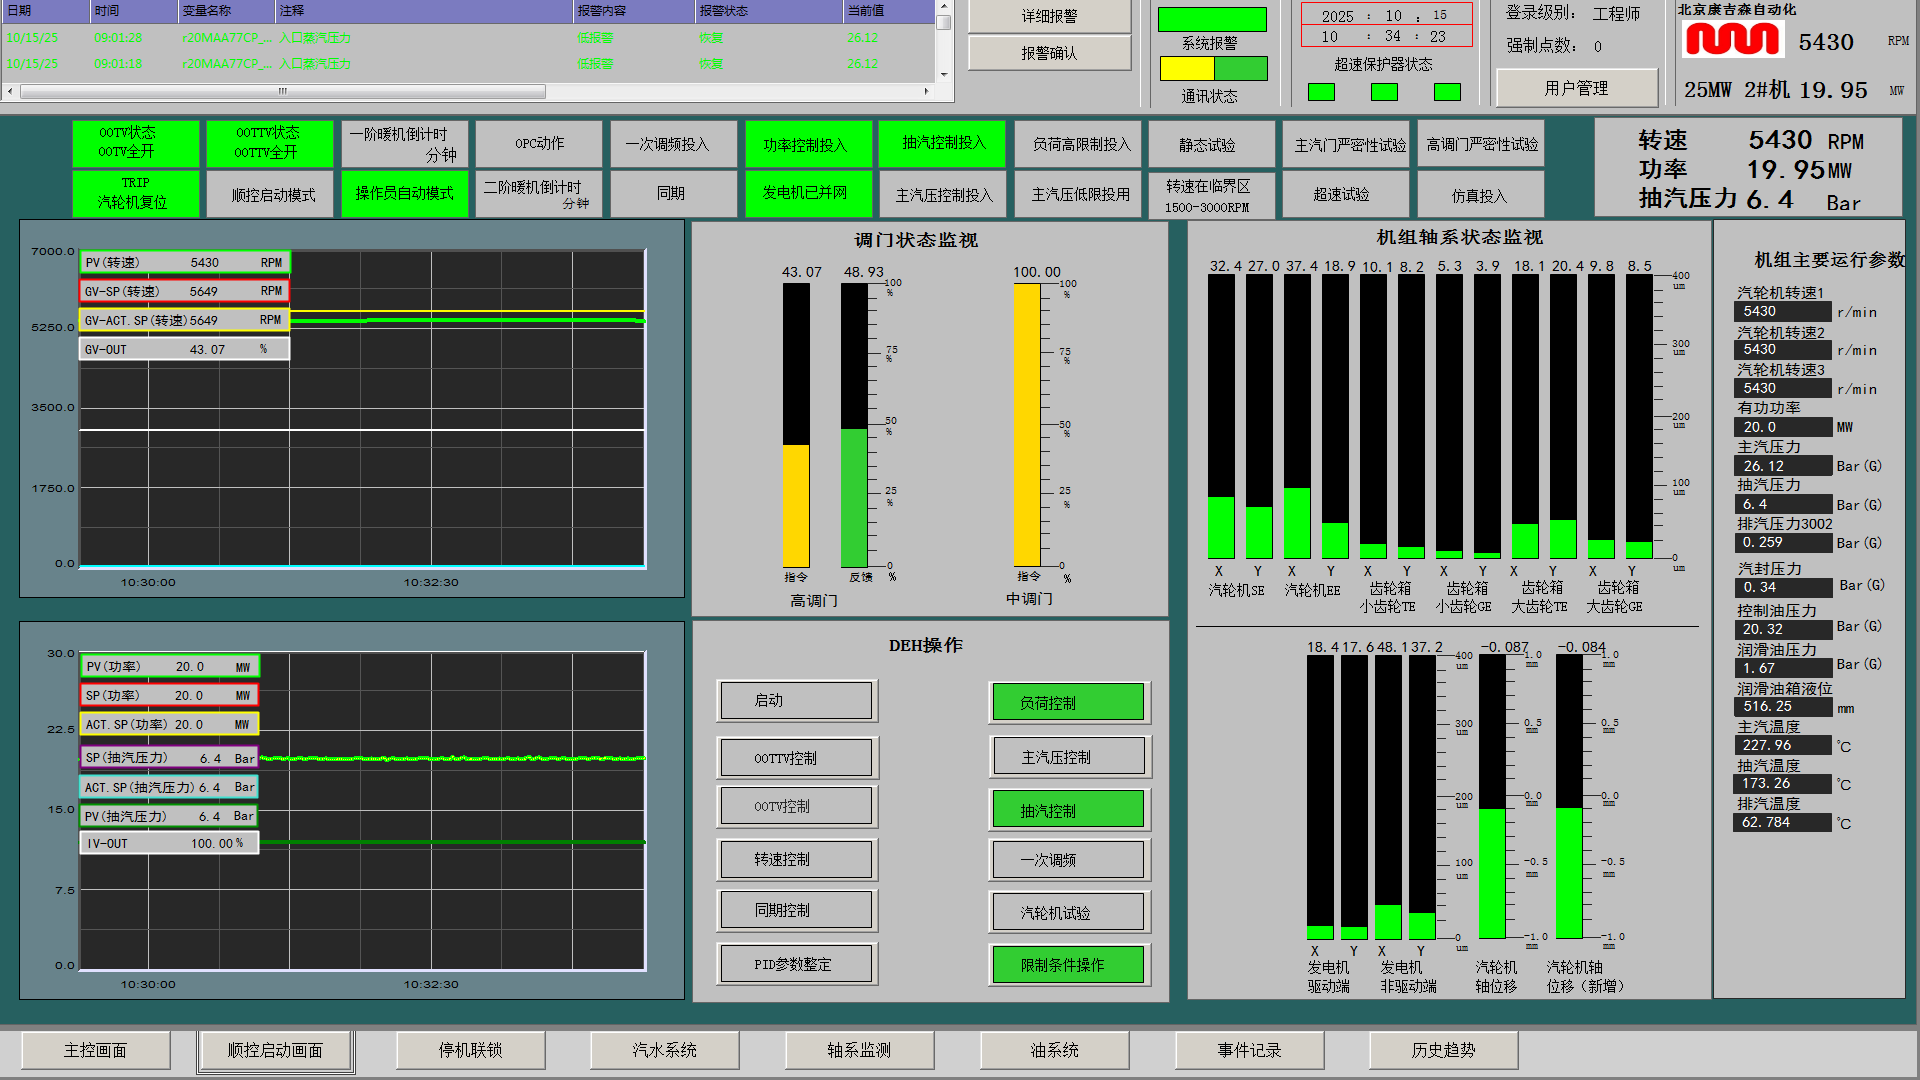
\includegraphics[width=300pt,keepaspectratio]{pic/zhu.png}
\caption{1号汽轮机DEH主控画面}
\label{fig:myphoto}
\end{figure}
	\end{frame}
\begin{frame}{1号汽轮机主控画面状态}{系统状态及汽轮机关键参数}
\begin{block}{DEH系统状态介绍}
			\begin{enumerate}
				\item 系统报警
				\item 通讯状态
			\end{enumerate}
		\end{block}
\begin{block}{汽轮机状态介绍}
			\begin{enumerate}
				\item 超速保护器状态
				\item OOTTV状态
				\item OOTV状态
				\item TRIP动作状态
				\item 发电机并网状态
			\end{enumerate}
		\end{block}
\end{frame}
\begin{frame}{1号汽轮机主控画面状态}{汽轮机当前操作模式}
\begin{block}{DEH系统状态介绍}
			\begin{enumerate}
				\item 转速控制投入
				\item 功率控制投入
				\item 抽汽控制投入
				\item 压力控制投入
			\end{enumerate}
		\end{block}
\begin{block}{DEH系统状态介绍}
			\begin{enumerate}
				\item OPC动作:转速大于103或并网信号消失
				\item 转速在临界区:转速在1500到3000rpm,升速率默认
			\end{enumerate}
		\end{block}
\end{frame}
\begin{frame}{1号汽轮机DEH操作介绍}{汽轮机启动}
  		\begin{columns}
			\column{.5\textwidth}
\begin{figure}
%\centering
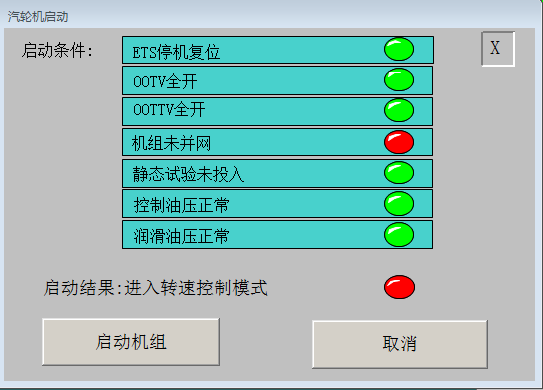
\includegraphics[angle=0,width=150pt,trim=0 0 0 0,clip]{pic/qidong.png}\\
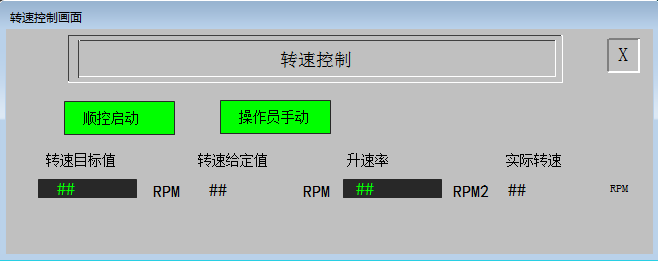
\includegraphics[angle=0,width=150pt,trim=0 0 0 0,clip]{pic/zhuansukongzhi.png}
%\caption{两线制接线图}
	
\end{figure}
	\column{.5\textwidth}
\begin{block}{汽轮机启动允许条件}
			\begin{enumerate}
				\item OOTV全开
				\item OOTTV全开
				\item 控制油压正常
				\item 润滑油压正常
				\end{enumerate}
\end{block}
\begin{exampleblock}{启动操作}
			\begin{enumerate}
				\item 按下启动机组按钮
				\item 机组进入转速控制模式
				\item 根据规程开始冲转暖机
				\end{enumerate}
\end{exampleblock}
		\end{columns}
\end{frame}
\begin{frame}{1号汽轮机DEH操作介绍}{汽轮机静态阀门试验}
  		\begin{columns}
			\column{.5\textwidth}
\begin{figure}
%\centering
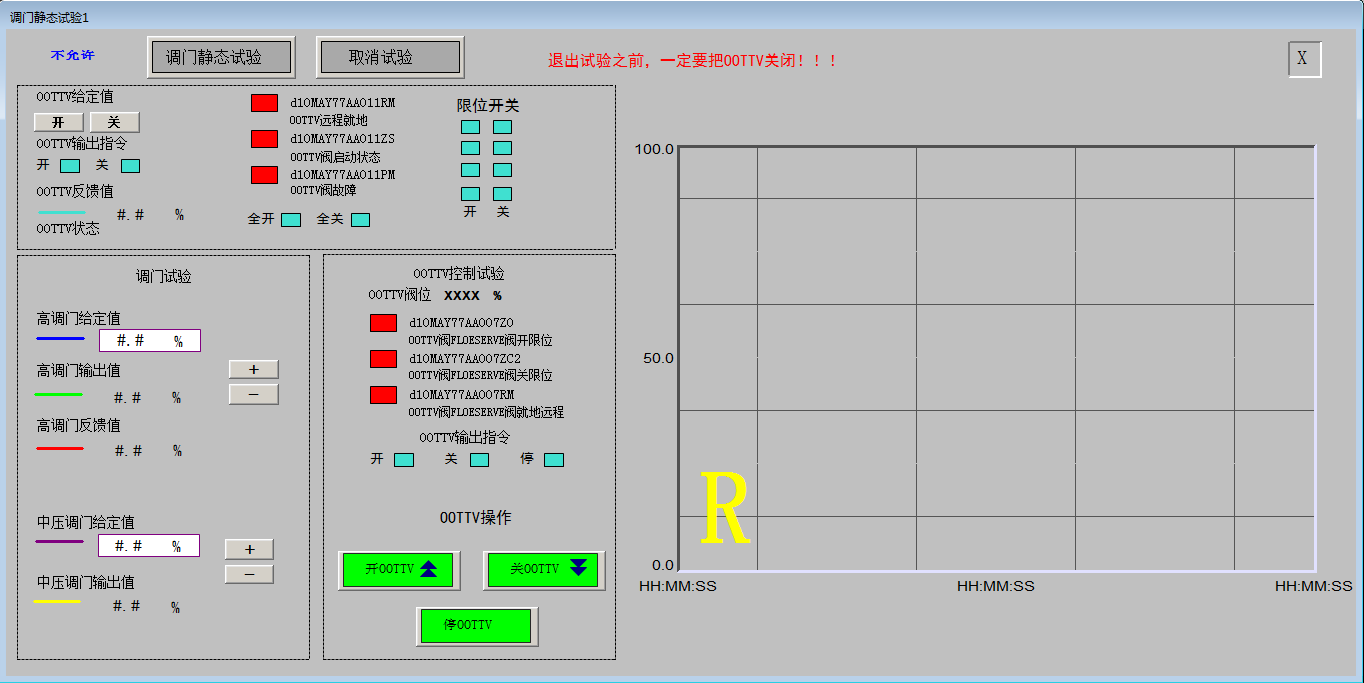
\includegraphics[angle=0,width=150pt,trim=0 0 0 0,clip]{pic/tiaomenjingtaishiyan.png}
%\caption{两线制接线图}
	
\end{figure}
	\column{.5\textwidth}
\begin{block}{高调门拉阀试验}
			\begin{enumerate}
				\item  与预先去皮比较的皮重偏差
				\item  总皮重值相对于额定负荷
				\end{enumerate}
\end{block}
\begin{block}{调门拉阀试验}
			\begin{description}
				\item[小于?]修正P04.05
				\item[大于?]超出允许误差
				\end{description}
\end{block}
\begin{alertblock}{注意!!}
			
				按下确认自动修改P04.05
\end{alertblock}
		\end{columns}
\end{frame}
\begin{frame}{1号汽轮机DEH操作介绍}{汽轮机左右导汽管阀门操作}
  		\begin{columns}
			\column{.5\textwidth}
\begin{figure}
%\centering
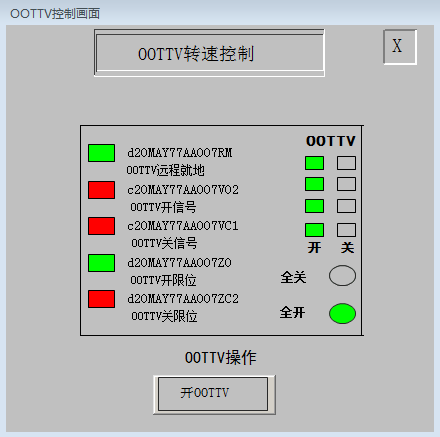
\includegraphics[angle=0,width=150pt,trim=0 0 0 0,clip]{pic/oottv.png}\\
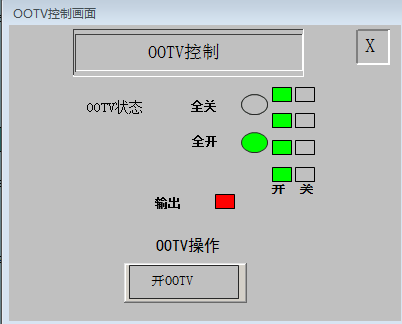
\includegraphics[angle=0,width=150pt,trim=0 0 0 0,clip]{pic/ootv.png}
%\caption{两线制接线图}
	
\end{figure}
	\column{.5\textwidth}
\begin{block}{回路特点}
			\begin{enumerate}
				\item  与预先去皮比较的皮重偏差
				\item  总皮重值相对于额定负荷
				\end{enumerate}
\end{block}
\begin{exampleblock}{标定结果评估}
			\begin{description}
				\item[小于?]修正P04.05
				\item[大于?]超出允许误差
				\end{description}
\end{exampleblock}
\begin{alertblock}{注意!!}
			
				按下确认自动修改P04.05
\end{alertblock}
		\end{columns}
\end{frame}
\begin{frame}{1号汽轮机DEH操作介绍}{汽轮机并网后负荷控制}
  		\begin{columns}
			\column{.5\textwidth}
\begin{figure}
%\centering
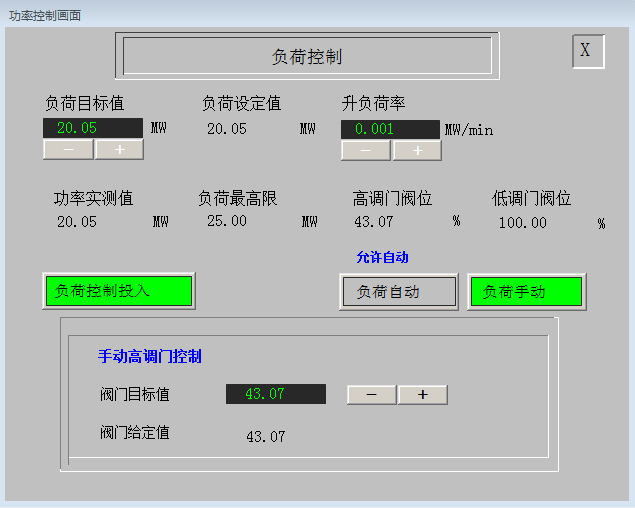
\includegraphics[angle=0,width=150pt,trim=0 0 0 0,clip]{pic/fuhe.png}
%\caption{两线制接线图}
	
\end{figure}
	\column{.5\textwidth}
\begin{block}{回路特点}
			\begin{enumerate}
				\item  与预先去皮比较的皮重偏差
				\item  总皮重值相对于额定负荷
				\end{enumerate}
\end{block}
\begin{exampleblock}{标定结果评估}
			\begin{description}
				\item[小于?]修正P04.05
				\item[大于?]超出允许误差
				\end{description}
\end{exampleblock}
\begin{alertblock}{注意!!}
			
				按下确认自动修改P04.05
\end{alertblock}
		\end{columns}
\end{frame}
\section{DEH系统设备讲解}
\subsection{系统转速}
\begin{frame}{汽轮机转速}{1号汽轮机转速采集}
\begin{block}{超速保护器转速采集}
			\begin{enumerate}
				\item 转速卡
				\item 继电器卡
				\item 模拟量输出卡
			\end{enumerate}
		\end{block}
\begin{block}{DEH系统转速采集}
			\begin{enumerate}
				\item PI开采集生成转速
				\item 系统转速
			\end{enumerate}
		\end{block}

\end{frame}
\begin{frame}{汽轮机转速}{4号汽轮机转速采集}
\begin{block}{TSI系统转速采集}
			\begin{enumerate}
				\item 6500转速卡
			\end{enumerate}
		\end{block}
\begin{block}{DEH系统转速采集}
			\begin{enumerate}
				\item 转速卡采集生成转速
				\item 系统转速生成
			\end{enumerate}
		\end{block}

\end{frame}
\subsection{高调门控制}
\begin{frame}{高调门控制}{1号汽轮机伺服阀开环控制}
\begin{block}{伺服阀信号控制}
			\begin{enumerate}
				\item 阀位指令:20-160mA指令
				\item  无阀位反馈,靠油缸动态平衡
			\end{enumerate}
		\end{block}
\pause
\begin{alertblock}{\heiti 开环控制!!!}
			无LVDT参与阀位控制 
		\end{alertblock}
\end{frame}
\begin{frame}{高调门控制}{3号汽轮机伺服阀}
\begin{block}{伺服阀信号控制}
			\begin{enumerate}
				\item 阀位指令:20-160mA指令
				\item  伺服卡
			\end{enumerate}
		\end{block}
\pause
\begin{alertblock}{\heiti 开环控制!!!}
			无LVDT参与阀位控制 
		\end{alertblock}
\end{frame}
\begin{frame}{高调门控制}{4号汽轮机伺服阀}
\begin{block}{伺服阀信号控制}
			\begin{enumerate}
				\item 阀位指令:20-160mA指令
				\item  伺服卡
			\end{enumerate}
		\end{block}
\pause
\begin{alertblock}{\heiti 开环控制!!!}
			无LVDT参与阀位控制 
		\end{alertblock}
\end{frame}
\section{DEH系统功能}
\subsection{超速保护}
\begin{frame}{超速保护}{1号汽轮机超速}
\begin{block}{\heiti 1号汽轮机DEH请求停机中电超速保护动作条件}
				主控超速110打闸:系统转速大于5975
		\end{block}
\begin{block}{\heiti 1号汽轮机ETS超速保护动作条件}
				超速保护器开关量信号三取二
		\end{block}
\begin{alertblock}{\heiti 超速保护器动作信号为故障安全型!!!}
			\begin{enumerate}
				\item 超速保护器开关量正常转速下是1,转速高于5975变为0
				\item 故障安全型信号优缺点
				\item 超速保护器转速监测
			\end{enumerate}
	\end{alertblock}
\end{frame}
\begin{frame}{超速保护}{3号汽轮机超速}
\begin{block}{\heiti 3号汽轮机DEH请求停机中超速保护动作条件}
				主控超速110打闸:系统转速大于5975
		\end{block}
\begin{block}{\heiti 3号汽轮机ETS超速保护动作条件}
				超速保护器开关量信号三取三且DEH转速任意一个转速大于4381
		\end{block}
\begin{alertblock}{\heiti ETS超速停机保护!!!}
			\begin{enumerate}
				\item 超速保护器开关量正常转速下是1,转速高于4381变为0
				\item 导致ETS超速停机条件如此的原因
			\end{enumerate}
	\end{alertblock}
\end{frame}
\begin{frame}{超速保护}{4号汽轮机超速}
\begin{block}{\heiti 4号汽轮机DEH请求停机中电超速保护动作条件}
			\begin{enumerate}
				\item  主控超速110打闸:系统转速大于3300
				\item  测速板超速110打闸:转速卡超速动作信号三取二
		\end{enumerate}
		\end{block}
\begin{block}{\heiti 4号汽轮机ETS超速保护动作条件}
				TSI系统转速卡动作信号三取二
		\end{block}
\end{frame}
\begin{frame}{超速保护}{1号汽轮机OPC超速保护}
\begin{block}{\heiti 1号汽轮机OPC保护动作条件}
			\begin{enumerate}
				\item 未并网前,系统转速大于
				\item 油开关跳闸:并网信号消失瞬间,功率大于7.5Kw,触发OPC动作
		\end{enumerate}
		\end{block}
\begin{block}{\heiti 1号汽轮机OPC保护复位条件}
			\begin{enumerate}
				\item 系统转速小于
				\item OPC触发两秒后复位
		\end{enumerate}
		\end{block}
\begin{block}{\heiti 1号汽轮机OPC保护动作设备}
			\begin{enumerate}
				\item 高调门全关
				\item 中调门全关
		\end{enumerate}
		\end{block}
\end{frame}
\begin{frame}{超速保护}{3号汽轮机OPC超速保护}
\begin{block}{\heiti 3号汽轮机OPC保护动作条件}
			\begin{enumerate}
				\item 未并网前,系统转速大于
				\item 油开关跳闸:并网信号消失瞬间,功率大于7.5Kw,触发OPC动作
		\end{enumerate}
		\end{block}
\begin{block}{\heiti 1号汽轮机OPC保护复位条件}
			\begin{enumerate}
				\item 系统转速小于
				\item OPC触发两秒后复位
		\end{enumerate}
		\end{block}
\begin{block}{\heiti 4号汽轮机OPC保护动作设备}
			\begin{enumerate}
				\item 高调门全关
		\end{enumerate}
		\end{block}
\end{frame}
\begin{frame}{超速保护}{4号汽轮机OPC超速保护}
\begin{block}{\heiti 4号汽轮机OPC保护动作条件}
			\begin{enumerate}
				\item 主控超速103
				\item 油开关跳闸
		\end{enumerate}
		\end{block}
\begin{block}{\heiti 4号汽轮机OPC保护复位条件}
			\begin{enumerate}
				\item 系统转速大于
				\item 并网信号消失瞬间,功率大于7.5Kw,触发OPC动作
		\end{enumerate}
		\end{block}
\begin{block}{\heiti 1号汽轮机OPC保护动作设备}
			\begin{enumerate}
				\item OPC电磁阀动作
				\item 中调门全关
				\item 高调门全关
		\end{enumerate}
		\end{block}
\end{frame}
\subsection{转速控制}
\begin{frame}{转速控制}{1号汽轮机转速控制}
\begin{block}{\heiti 1号汽轮机启动允许条件}
			\begin{enumerate}
				\item OOTTV和OOTV全开
				\item 控制油压力和润滑油压力正常
				\item ETS停机复位机组未并网静态试验未投入
		\end{enumerate}
		\end{block}
\begin{block}{\heiti 目标转速和升速率设置}
			\begin{enumerate}
				\item 临界转速升速率
		\end{enumerate}
		\end{block}
\begin{block}{\heiti 定速后并网设置}
			\begin{enumerate}
				\item 并网瞬间高调门开度增加3.5
		\end{enumerate}
		\end{block}
\end{frame}
\begin{frame}{转速控制}{3号汽轮机阀门切换}
\begin{block}{\heiti 3号汽轮机启动允许条件}
			\begin{enumerate}
				\item OOTTV和OOTV全开
				\item 控制油压力和润滑油压力正常
				\item ETS停机复位机组未并网静态试验未投入
		\end{enumerate}
		\end{block}
\begin{block}{\heiti 目标转速和升速率设置}
			\begin{enumerate}
				\item 临界转速升速率
		\end{enumerate}
		\end{block}
\begin{block}{\heiti 定速后并网设置}
			\begin{enumerate}
				\item 并网瞬间高调门开度增加3.5
		\end{enumerate}
		\end{block}
\end{frame}
\begin{frame}{转速控制}{3号汽轮机转速控制}
\begin{block}{\heiti 3号汽轮机启动允许条件}
			\begin{enumerate}
				\item OOTTV和OOTV全开
				\item 控制油压力和润滑油压力正常
				\item ETS停机复位机组未并网静态试验未投入
		\end{enumerate}
		\end{block}
\begin{block}{\heiti 目标转速和升速率设置}
			\begin{enumerate}
				\item 临界转速升速率
		\end{enumerate}
		\end{block}
\begin{block}{\heiti 定速后并网设置}
			\begin{enumerate}
				\item 并网瞬间高调门开度增加3.5
		\end{enumerate}
		\end{block}
\end{frame}
\subsection{在线试验}
\begin{frame}{1号汽轮机DEH操作介绍}{汽轮机静态阀门试验}
  		\begin{columns}
			\column{.5\textwidth}
\begin{figure}
%\centering
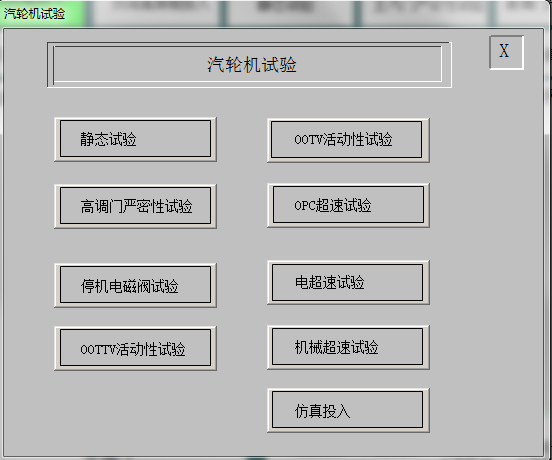
\includegraphics[angle=0,width=150pt,trim=0 0 0 0,clip]{pic/shiyan.png}
%\caption{两线制接线图}
	
\end{figure}
	\column{.5\textwidth}
\begin{block}{回路特点}
			\begin{enumerate}
				\item  与预先去皮比较的皮重偏差
				\item  总皮重值相对于额定负荷
				\end{enumerate}
\end{block}
\begin{exampleblock}{标定结果评估}
			\begin{description}
				\item[小于?]修正P04.05
				\item[大于?]超出允许误差
				\end{description}
\end{exampleblock}
\begin{alertblock}{注意!!}
			
				按下确认自动修改P04.05
\end{alertblock}
		\end{columns}
\end{frame}
\begin{frame}{我厂DCS系统架构实例}{重要辅机系统在控制器内分布情况}
\begin{block}{\heiti 分散布置的系统}
			\begin{enumerate}

				\item  六大风机、空预器、制粉系统分为两组分别分布在两组控制器
				
				\item   4台电动给水泵系统分为两组分别分布在两组控制器
		\end{enumerate}
		\end{block}
\pause
\begin{alertblock}{\heiti 存在问题}
			\begin{enumerate}
				\item  设备分散不彻底,锅炉侧调门、变频器在同一台控制器
				
				\item  主设备停运后触发MFT信号集中在同一台控制器
		\end{enumerate}
		\end{alertblock}
\end{frame}

\begin{frame}{我厂DCS系统架构实例}{重要辅机系统在控制器内分布情况}
\begin{exampleblock}{\heiti 分布在一台控制器}
			\begin{enumerate}
				\item  六大风机入口调门和变频器、4台制粉系统冷热风调门和给煤机变频器、主/辅给水调门
				
				\item  3组高加系统、4组除氧器系统
				
				\item   1、2、3号汽轮机凝结水泵、空冷风机

				\item   4、5号汽轮机控制油泵、润滑油泵、凝结水泵、空冷风机
		\end{enumerate}
		\end{exampleblock}
\pause
\begin{alertblock}{\heiti 风险}
			\begin{enumerate}
				\item  一组控制器故障会影响所有设备!
\item  如果必须执行初始化下装,所有设备会恢复初始状态!
		\end{enumerate}
		\end{alertblock}
\end{frame}
\subsection{重要测点在I/O模件内分布情况}

\begin{frame}{我厂DCS系统架构实例}{重要测点在I/O模件内分布情况}
\begin{alertblock}{\heiti 保护测点分布在同一块卡件}
			\begin{enumerate}
				\item  炉膛压力高高、炉膛压力低低测点
			
		\end{enumerate}
		\end{alertblock}
\pause
\begin{alertblock}{\heiti 调门或变频器指令分布在同一块卡件}
			\begin{enumerate}
				\item  管网双减调节阀指令
				\item  除氧器压力、液位、高压加热器液位调节阀指令
				\item 六大风机入口调门、磨煤机冷热风调门、给煤机指令
			
		\end{enumerate}
		\end{alertblock}
\begin{alertblock}{\heiti DO通道配置有长电平指令设备}
			\begin{enumerate}
				\item  六大风机、空预器、制粉系统停运触发MFT信号
			
		\end{enumerate}
		\end{alertblock}
\end{frame}
\begin{frame}

\begin{table}
	\caption{800XA故障试验结果}
	\begin{tabular}{|c|c|c|c|c|}
		\hline
		       操作    & AI         & DI     & AO&DO  \\   \hline
		卡件故障    & 保持        & 保持      & 保持&保持  \\  \hline 
		更换卡件    & 保持    & 保持   & 复位&复位\\  \hline  
		通讯电缆故障    & 保持        & 保持      & 保持& 保持 \\   \hline  
		站头故障    &保持          & 保持       & 保持& 保持 \\     \hline
CI854故障    &保持          & 保持       & 保持& 保持 \\     \hline
控制器故障    &保持          & 保持       & 保持& 保持 \\     \hline
初始化下装    &复位          & 复位       & 复位& 复位 \\     \hline
	\end{tabular}
	\end{table}
注:站头CI840同时拔出后下属卡件值都会复位


\end{frame}
%\section{DCS典型案例}
\begin{frame}{DCS典型案例}{C3控制器故障处理导致1号锅炉停运}
\begin{block}{\heiti 控制器初始化下装导致锅炉灭火}
			CEX电缆松动导致两台控制器故障且控制器内程序丢失,需要初始化下装逻辑后才能正常运行,将相关设备切至就地后进行初始化下装,下装过程中3台风机变频器跳闸触发炉膛压力低低保护。
		\end{block}
\pause
\begin{alertblock}{\heiti DO电平指令初始化下装过程中复位为0}
			
				检查为风机变频器有软急停电平指令接至DCS DO通道,指令变为0时变频器急停。
			
		
		\end{alertblock}
\end{frame}
\begin{frame}{DCS典型案例}{净化装置控制器故障处理导致全厂停运}
\begin{block}{\heiti 控制器初始化下装导致停车}
			两台控制器故障且控制器内程序丢失,需要初始化下装逻辑后才能正常运行,下装过程调门关闭导致停车
		\end{block}
\pause
\begin{alertblock}{\heiti AO指令初始化下装过程中复位为0}
			
				调节阀指令恢复为0导致调节阀关闭,系统停车
			
		
		\end{alertblock}
\end{frame}
\begin{frame}{DCS典型案例}{所有上位机失电导致工况无法监控调整30分钟}
\begin{block}{\heiti 所有上位机失电导致工况无法监控调整}
			因电气误停UPS电源导致DCS系统公用总电源失电后,所有上位机失电,操作员站、工程师站、各服务器失电导致工况无法监控调整,陆续恢复电源并恢复服务器和操作员站后工况稳定无影响。
		\end{block}
\pause
\begin{alertblock}{\heiti 怎么做???风险!!!
}
			
				紧急停运,停运措施是否完整,风险?\\继续运行,工况是否平稳,风险?
			
		
		\end{alertblock}
\end{frame}

\section{存在的问题与做什么}
\begin{frame}{存在的问题与做什么}{存在的问题}
\begin{alertblock}{\heiti 目前存在问题!!!}
			\begin{enumerate}
				\item  CEX电缆松动会导致一组控制器内程序清空
\item  重要调门集中在同一组控制器上
\item  重要调门AO指令在同一块卡件上未分散
				\item  重要辅机对应控制器故障后具体的处理细节
\item  服务器、工作站备份恢复无法实现
				
				\item  800XA系统各状态有效的监视手段

				\item  网络变量、全局变量的合理使用

				
\item  AO卡件故障后现场对应启动调门应该采取什么措施
		\end{enumerate}
		\end{alertblock}
\end{frame}
\begin{frame}{存在的问题与做什么}{做什么}
\begin{alertblock}{\heiti 下一步做什么???}
			\begin{enumerate}
				\item  合理布置AO调门指令分布
				\item   对现场设备AO、DO指令情况进行具体排查分类确认故障及处理过程中应对措施
\item   DCS系统指令复位时各专业如何保证现场设备保持原状态
				\item   实现备份、恢复服务器
				\item   利用现有备件搭建一套单节点系统


		\end{enumerate}
		\end{alertblock}
\end{frame}


	
	

	
\begin{frame}{排查内容}{排查清单}  
 \begin{thebibliography}{99}

\bibitem{AO} AO指令: \emph{ABB系统AO点排查},
热控专业, 2023-11-16
\bibitem{DO} DO指令: \emph{ABB系统DO点排查},
热控专业, 2023-11-16
\bibitem{AO} 气动调门: \emph{AO供电调节阀},
热控专业, 2023-11-16
\bibitem{AO} 变频器: \emph{变频器远方就地切换状态},
电气专业, 2023-11-16
\end{thebibliography}
\end{frame}
\end{document}
